\documentclass[onecolumn, 12pt]{article}
\usepackage{fullpage}
\usepackage{graphicx}
\usepackage{setspace}
\doublespacing

\title{}
\author{Matthew Gardner}
\date{}

\begin{document}

\textbf{Art Response}

\begin{tabular}{ll}
  Name:&Matthew Gardner \\
  Work:&Levers, Ramps and Pulleys \\
  Artist:&Walter Wick \\
  Date:&1995 \\
\end{tabular}

\section*{Historical Context}

Walter Wick is the artist and photographer who produced the popular \emph{I
Spy} books.  He was born in Hartford, Connecticut in 1953.  His early career
was in commercial photography, and he quickly ended up doing photo-illustration
for books and creating photographic puzzles and optical illusions.  The \emph{I
Spy} books stem from his work as a photographer.  For many of the pictures used
in his books, he created complex scenes, either of toys or of miniatures or
whatever he needed, and photographed them.  The series of eight books sold over
a million copies.  \emph{Levers, Ramps and Pulleys} was originally published in
\emph{I Spy: School Days}.

\section*{Critical Analysis}

\emph{Levers, Ramps and Pulleys} is a fun photograph of a balloon popper that
Walter Wick constructed.  Hitting on an oft-used theme, Wick creates his
balloon popper as an immensely complicated contraption, where starting one
little thing in motion causes another to move, and so on, until some result is
achieved, in this case popping a balloon.  Wick didn't just make any old
contraption for his balloon popper, however; he clearly understood the
principles of good art and used them in his piece.  The structure of the
popper, the extra items included in the picture, and its playful character all
give the piece an added depth and evoke a strong emotional response from the
viewer.

The contraption starts in the top left corner of the photograph.  Following the
path of the ball after it is set in motion leads one across the page and down,
following clear lines that draw the viewer's eyes from the beginning to the
balloon in the lower right corner.  While what's going on is somewhat
complicated, the general path the motion takes is easy to follow, and the
details give viewers places to pause and delight in Wick's ingenuity.  Also
cleverly placed at the conclusion of the motion is the ``scoreboard,'' showing
a tally of successful vs. failed attempts at popping the balloon.  The way the
photograph is structured shows the careful planning that went into its
production.

There is a lot going on in \emph{Levers, Ramps and Pulleys}.  A large portion
of the materials seen in the photograph are part of the balloon popper, but
there are also a number of toys and other objects that don't appear to have any
purpose in being there.  However, in addition to filling up some blank space
that would otherwise have been in the picture, they bring images to the viewer
of the process that Wick went through in creating his popper.  There are
scissors left open as if recently used to cut the pieces of string found in the
contraption.  The source of the sand used in the balloon popper is readily
found to be the large bucket of sand that is missing a scoop.  The tally in the
corner leaves one wondering if the other pieces were used in the failed
attempts, but were replaced and left aside when Wick found that they failed in
their part of the contraption.  Wick's inclusion of extra items in his piece
greatly enhances the character of the photograph.

Every child plays with toys, and there aren't many that do not line up dominoes
to knock over at some point in their lives.  Wick's use of common children's
toys in his contraption make the piece approachable by younger audiences and
adorable to adults.  For children, the photograph likely makes stirs their
imagination, making them think of all of the fun and interesting contraptions
\emph{they} could build with the toys they have.  In adults, the piece brings
back childhood memories, or perhaps recent memories of playing with their
children.  Whoever the audience, Wick's picture is evocative and fun.

\emph{Levers, Ramps and Pulleys} is a playful work of ingenuity.  Not only is
it entertaining to look at, it demonstrates Wick's understanding of his
audience, young and old, and his grasp of artistic principles.  It is a
masterpiece of modern photography.

\section*{Personal Reflection}

\emph{Levers, Ramps and Pulleys} was really fun for me to see.  I find Wick's
work fascinating.  I always enjoyed building things with Tinker Toys, blocks,
and dominoes, so the piece really resonated with me.  I have never been very
good at analyzing artwork, however, so trying to find something to write about
was difficult for me.  But I found that as I spent time thinking about
different characteristics of the piece, I appreciated it a lot more.  Noticing
the motion in the picture and thinking about the purpose of the extra elements
why the tally was there were very rewarding.  And in the extra reading I did
when preparing to write my response I found a video on the contraption working
on Walter Wick's website, walterwick.com.  That, of course, was the best part
of the whole process.

\begin{center}
  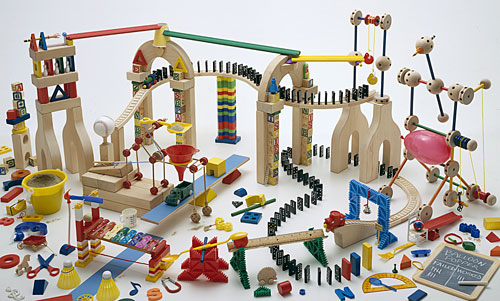
\includegraphics[width=.5\textwidth]{levers.jpg}
\end{center}

\end{document}
